% !Mode:: "TeX:UTF-8"
\documentclass[landscape]{article}
%\documentclass[10pt,portrait]{article}
\usepackage{pslatex}
\usepackage{graphicx}
\usepackage{multicol}
\usepackage{calc}
\usepackage{color}
\usepackage{amssymb, amsmath, amsfonts}
\usepackage{picins}
\usepackage{url}
\usepackage{tabularx,multicol}
\usepackage{array,booktabs,textcomp}
\renewcommand\baselinestretch{1.1}  %% 全局控制行间距

\usepackage[slantfont, boldfont]{xeCJK}

%% 针对中文进行断行
\XeTeXlinebreaklocale "zh"

%% 给予TeX断行一定自由度
\XeTeXlinebreakskip = 0pt plus 1pt minus 0.1pt

%%%% xeCJK设置结束

%% 设置缺省中文字体
\setCJKmainfont{NotoSansSC-Regular}
%% 设置中文无衬线字体
%\setCJKsansfont[Scale=0.8]{宋体}
%% 设置等宽字体
\setCJKmonofont[Scale=0.7]{NotoSansSC-Regular}

%% 英文衬线字体
\setmainfont{CMU Serif}
%% 英文等宽字体
\setmonofont[Scale=0.8]{Courier New} % 对verbatim内代码格式有效
%% 英文无衬线字体
\setsansfont[Scale=1]{Candara}  % 对公式有效

% Turn off header and footer
\pagestyle{empty}

%\setlength{\leftmargin}{0.75in}
\setlength{\oddsidemargin}{-0.75in}
\setlength{\evensidemargin}{-0.75in}
\setlength{\textwidth}{10.5in}


\setlength{\topmargin}{-0.2in}
\setlength{\textheight}{7.4in}
\setlength{\headheight}{0in}
\setlength{\headsep}{0in}

\pdfpageheight\paperheight
\pdfpagewidth\paperwidth


% Redefine section commands to use less space
\makeatletter
\renewcommand\section{\@startsection{section}{1}{0mm}%
                                     {0.5ex}% \@plus -12pt \@minus -6pt}%
                                     {0.5ex}%
                                {\color{black}\normalfont\large\bfseries}}
\makeatother

% Don't print section numbers
\setcounter{secnumdepth}{0}

\setlength{\parindent}{0pt}
\setlength{\parskip}{0pt}

\newcommand{\code}{\texttt}
\newcommand{\bcode}[1]{\texttt{\textbf{#1}}}
\renewcommand{\today}{\number\year 年 \number\month 月 \number\day 日}%重定义中文日期
%\newcommand\F{\code{FALSE}}
%\newcommand\T{\code{TRUE}}

%\newcommand{\hangpara}[2]{\hangindent#1\hangafter#2\noindent}
%\newenvironment{hangparas}[2]{\setlength{\parindent}{\z@}\everypar={\hangpara{#1}{#2}}}

\newcommand{\describe}[1]{\begin{description}{#1}\end{description}}

%\definecolor{steelblue}{rgb}{.6,0,0}
\definecolor{steelblue}{rgb}{0,0,0}

% -----------------------------------------------------------------------

\begin{document}

%\raggedright
\footnotesize
\begin{multicols*}{3}

% multicol parameters
% These lengths are set only within the two main columns
%\setlength{\columnseprule}{0.25pt}
\setlength{\premulticols}{1pt}
\setlength{\postmulticols}{1pt}
\setlength{\multicolsep}{1pt}
\setlength{\columnsep}{2pt}

\begin{center}
%    \Large{\textbf{\color{blue}R Reference Card}} \\
     \Large{\textbf{\color{blue}R 参考卡片}} \\
\end{center}
%by Tom Short, EPRI Solutions, Inc., tshort@eprisolutions.com
%2004-10-21 \\
%translated by SZ Liu, sunbjt@hotmail.com    2006-09-22\\
%Granted to the public domain. See www.Rpad.org for the source and latest version.
%Includes material from \emph{R for Beginners} by Emmanuel Paradis (with permission).\\
原文档由 ~Tom Short~撰写,你可以在 \url{www.Rpad.org} 上得到最新文档。
中文版本文档 (已获得Tom Short的翻译许可)结构上同原版类似,局部添加了若干常用命令。后续修订以及维护由刘思喆负责。

%version~1.0~   2006-09-22
项目同步在这里 \url{https://github.com/sunbjt/r_reference}

update:\today


%\section{Getting help}
\section{帮助和基础}
\everypar={\hangindent=7mm}

%Most R functions have online documentation.
大部分 R 函数都有在线文档。

%\bcode{help(topic)} documentation on \code{topic}
\bcode{help(topic)} 关于 \code{topic}的文档.

%\bcode{?topic} id.
\bcode{?topic} 同上

%\bcode{help.search("topic")} search the help system
\bcode{help.search("topic")} 搜索帮助系统

%\bcode{apropos("topic")} the names of all objects in the search list
%matching the regular expression "topic"
\bcode{apropos("topic")} 返回在搜索路径下包含(部分)关键词"topic"的所有对象名称


%\bcode{help.start()} start the HTML version of help
\bcode{help.start()} HTML形式的帮助

%\bcode{demo}   Demonstrations of R Functionality
\bcode{demo()}    ~R~功能演示

%\bcode{example(f)}  Run an Examples Section from the Online Help
\bcode{example(f)}  运行在线帮助中的例子

%\bcode{str(a)} display the internal *str*ucture of an R object
\bcode{str(a)} 显示 R 对象的内在属性(*str*ucture)或简要说明对象

%\bcode{summary(a)} gives a 'summary' of \code{a}, usually a
%statistical summary but it is \emph{generic} meaning it has different operations for different
%classes of \code{a}
\bcode{summary(a)} 给出 \code{a}的概要, 通常是一个一般性统计概要;且它对不同属性的 \code{a} 有不同的操作方式.

%\bcode{ls()} show objects in the search path; specify \code{pat="pat"}
%to search on a pattern
\bcode{ls()} 显示'搜索路径'下的对象; 也可按指定条件搜索。

%\bcode{ls.str()} str() for each variable in the search path
\bcode{ls.str()} str() 搜索路径下的每个变量与其属性

%\bcode{dir()} show files in the current directory
\bcode{dir()} 显示当前目录下的文件

\bcode{list.files()}    同上

\bcode{getwd()} 获得工作路径信息

\bcode{setwd()} 设置工作路径

%\bcode{methods(a)} shows S3 methods of \code{a}
\bcode{methods(a)}  显示\code{a}的'S3 methods'

%\bcode{methods(class=class(a))} lists all the methods to handle objects
%of class a
\bcode{methods(class=class(a))} 列表所有可以解决属于对象类的方法

%\bcode{options(...)} set or examine many global options; common ones:
%\code{width}, \code{digits}, \code{error}
\bcode{options(...)} 设置或检验全局参数; 常用参数有:
\code{width}, \code{digits}, \code{error}

\bcode{install.packages(pkg)} 安装 pkg 包

\bcode{update.packages()} 自动对比包版本,并询问更新

%\bcode{library(x)} load add-on packages; \code{library(help=x)} lists
%datasets and functions in package \code{x}~.
\bcode{library(pkg)} 加载pkg包

\bcode{require(x)}  同上

\bcode{library(help=pkg)} 展示
包  \code{pkg} 的信息

%\bcode{attach(x)} database \code{x}~to the R search path;
%\code{x}~can be a list, data frame, or R data file created with
%\code{save}. Use \code{search()} to show the search path.
\bcode{attach(x)} 将 \code{x}~指向R的搜索路径;
\code{x}~可以使一个列表,数据框,或者是由 \code{save}创建的 R data file.
使用 \code{search()}来显示搜索路径.

%\bcode{detach(x)} \code{x}~from the R search path;
%\code{x}~can be a name or character string of an object previously
%attached or a package.
\bcode{detach(x)} \code{attach}的逆过程.

\bcode{assign(x,value)} 将\code{value}赋值给\code{x}~,即"$<-$"

\bcode{quit()}  退出当前~R~会话(q()或Ctrl\_z)


%\section{Input and output}
\section{输入与输出}

\everypar={\hangindent=9mm}

%\bcode{load()} load the datasets written with \code{save}
\bcode{load()} 加载由\code{save}命令得到的资料集

%\bcode{data(x)} loads specified data sets
\bcode{data(x)} 加载指定的数据

%\bcode(edit())Invoke a text editor on an R object.
\bcode{edit()}    调用文本编辑器修改R对象

%\bcode{fix(x)}       'fix' invokes 'edit' on 'x' and then assigns the new (edited)
%     version of 'x' in the user's workspace.
\bcode{fix(x)}  'fix' 调用 'edit' 修改 'x'

\bcode{data.entry(x)}  电子数据表形式的录入编辑器

\bcode{scan(x)} 从控制台或文件中读取数据为向量或列表

%\bcode{library(x)} load add-on packages
%\bcode{library(x),require(x)} 加载额外的包

%\bcode{read.table(file)} reads a file in table format and
%                creates a data frame from it; the default separator
%                \code{sep=""} is any whitespace; use \code{header=TRUE}
%                to read the first line as a header of column names; use \code{as.is=TRUE} to
%                prevent character vectors from being converted to
%                factors; use \code{comment.char=""} to prevent
%                \code{"\#"} from being interpreted as a comment; use
%                \code{skip=n} to skip \code{n} lines before reading data; see
%                the help for options on row naming, NA treatment, and
%                others
\bcode{read.table(file)} 读取表格式的文件并将其创建成数据框;默认分割符
                \code{sep=""}为任意空白;使用\code{header=TRUE}
                读取第一行作为列标题;使用\code{as.is=TRUE}防止字符向量变为
                factors;使用\code{comment.char=""}防止\code{"\#"}被解释为注释;
                使用\code{skip=n} 在读数据前跳过 \code{n} 行;详细见帮助关于行
                命名,NA 处理,和其他

%\bcode{read.csv("filename",header=TRUE)} id. but with defaults set for reading
%comma-delimited files
\bcode{read.csv("filename",header=TRUE)} 同上,但默认设置为读取~\code{csv} 文件(Comma Separated values)

%\bcode{read.delim("filename",header=TRUE)} id. but with defaults set for reading
%tab-delimited files
\bcode{read.delim("filename",header=TRUE)} 同上,默认设置为读取 \code{tab} 分割文件


%\bcode{read.fwf(file,widths,header=FALSE,sep="\t",as.is=FALSE)} read a table of
%\emph{f}ixed \emph{w}idth \emph{f}ormatted data into a
%     'data.frame'; \code{widths} is an integer vector, giving the widths of the fixed-width fields
\bcode{read.fwf(file,widths,header=F,sep="$\backslash$t",as.is=FALSE)}   \\
以fixed width formatted形式读取数据
至数据框; \code{widths} 是整数向量, 用于设置调整宽度字段

%\bcode{save(file,...)} saves the specified objects (...) in the XDR
%platform-independent binary format
\bcode{save(file,...)} 以不分平台的二进制保存指定的对象

%\bcode{save.image(file)} saves all objects
\bcode{save.image(file)} 保存所有的对象


\bcode{dump("x","...")}    将对象~x~保存在'...'里

%\bcode{cat(..., file="", sep=" ")} prints the arguments after coercing to
%character; \code{sep} is the character separator between arguments
\bcode{cat(..., file="", sep=" ")} 强制转化为字符后打印 对象的赋值;
                                     \code{sep} 为对象赋值间的分割符号

%\bcode{print(a, ...)} prints its arguments; generic, meaning it can
%have different methods for different objects
\bcode{print(a, ...)} 显示\code{a}的赋值,更一般的,它对于不同的对象可以有不同的表达方式。

%\bcode{format(x,...)} format an R object for pretty printing
\bcode{format(x,...)} 格式化,更好的显示 R 对象

%\bcode{write.table(x,file="",row.names=TRUE,col.names=TRUE, sep=" ")}
%prints \code{x}~after converting to a data frame; if \code{quote} is
%                 \code{TRUE}, character or factor columns are
%                 surrounded by quotes (\code{"}); \code{sep} is the field
%                 separator; \code{eol} is the end-of-line separator;
%                 \code{na} is the string for missing values; use
%                 \code{col.names=NA} to add a blank column header to
%                 get the column headers aligned correctly for
%                 spreadsheet input

\bcode{write.table(x,file="",row.names= T ,col.names= T , sep="")}
在把\code{x}~转化为数据框后,写到文件; 如果 \code{quote} 为
                 \code{TRUE}, 字符和因子列就会被 (\code{"})所包围; \code{sep} 是字段分隔符
                 ; \code{eol} 为尾行分割符;
                 \code{na} 为缺失值字符串; 使用
                 \code{col.names=NA} 增加列标题以便于和表格输入一致

%\bcode{sink(file)} output to \code{file}, until \code{sink()}
\bcode{sink(file)} 输出到文件\code{file}, 直到输入命令 \code{sink()}

\everypar={\hangindent=9mm}
%Most of the I/O functions have a \code{file} argument. This can often
%be a character string naming a file or a connection.  \code{file=""} means the standard input or
%output. Connections can include files, pipes, zipped
%files, and R variables.
\vspace{2mm}

大部分~$I/O$~函数都有 \code{file} 参量.它经常用一个字符串来命名文件或连接. \code{file=""} 意味着标准输入或输出.
连接(Connections)可以包含文件(file),管道(pipes),压缩文件(zipped files)或~R~变量

%On windows, the file connection can also be used with \code{description =
%"clipboard"}. To read a table copied from Excel, use \\
%\code{x <- read.delim("clipboard")}\\
%To write a table to the clipboard for Excel, use \\
%\code{write.table(x,"clipboard",sep="\textbackslash t",col.names=NA)}
在~windows~操作环境下,数据共享可以通过写字板(clipboard)的方式.读取~Excel~表:可以将~Excel~中数据拷贝至写字板
(内存),使用 \code{x <- read.delim('clipboard')} 方式读取数据。

\code{write.table(x, 'clipboard', sep='\t',col.names=NA)}可以将数据写入clipboard,可直接粘贴到Excel中。

%For database interaction, see packages \code{RODBC}, \code{DBI},
%\code{RMySQL}, \code{RPgSQL}, and \code{ROracle}. See packages \code{XML}, \code{hdf5}, \code{netCDF} for reading
%other file formats.
数据库方面的交互应用,请见 \code{RODBC}, \code{DBI},\code{RMySQL}, \code{RPgSQL}, and \code{ROracle}包.
读取其他文件格式参考 \code{XML}, \code{hdf5}, \code{netCDF} 等包.



%\section{Data creation}
\section{数据创建}
\everypar={\hangindent=9mm}

%\bcode{c(...)} generic function to combine arguments with the default
%forming a vector;
%with \code{recursive=TRUE} descends through lists combining all elements
%into one vector
\bcode{c(...)} 常见的将一系列参量转化为向量的函数;
通过 \code{recursive=TRUE} 降序排列列表并组合所有的元素为向量.

%\bcode{from:to} generates a sequence; ':' has operator priority; 1:4
%+ 1 is '2,3,4,5'
\bcode{from:to} 产生一个序列; ':' 有较高级别的优先级; 1:4
+ 1 得到 '2,3,4,5'

%\bcode{seq(from,to)} generates a sequence
\bcode{seq(from,to)} 产生一个序列
%\code{by=} specifies increment; \code{length=} specifies desired length
\code{by=} 指定间距; \code{length=} 指定要求长度

%\bcode{seq(along=x)} generates \code{1, 2, ..., length(along)}; useful for
%\code{for} loops

\bcode{seq(along=x)} 产生 \code{1, 2, ..., length(along)}; 常用在循环上

%\bcode{rep(x,times)} replicate \code{x}~\code{times}; use \code{each=}
%to repeat 'each' element of \code{x}~\code{each} times;
%\code{rep(c(1,2,3),2)} is 1 2 3 1 2 3; \code{rep(c(1,2,3),each=2)} is 1 1 2 2 3 3
\bcode{rep(x,times)} 重复 \code{x}~\code{times}次; 使用 \code{each=}
来指定元素 \code{x}~重复的次数;\code{rep(c(1,2,3),2)} 将得到 1 2 3 1 2 3;
\code{rep(c(1,2,3),each=2)} 将得到 1 1 2 2 3 3

%\bcode{data.frame(...)} create a data frame of the named or unnamed arguments;
%  \code{data.frame(v=1:4,ch=c("a","B","c","d"),n=10)}; shorter vectors
%  are recycled to the length of the longest
\bcode{data.frame(...)}  创建数据框,当然变量可能被命名或不被命名;
  \code{data.frame(v=1:4,ch=c("a","B","c","d"),n=10)}; 相对较短的向量会被循环填充到
  最长向量长度


%\bcode{list(...)} create a list of the named or unnamed arguments;
%  \code{list(a=c(1,2),b="hi",c=3i)};
\bcode{list(...)} 创建一个由变量组成的列表,变量可能被命名或未被命名;
  \code{list(a=c(1,2),b="hi",c=3i)};

%\bcode{array(x,dim=)} array with data \code{x}~; specify
%dimensions like \code{dim=c(3,4,2)}; elements of \code{x}~recycle if \code{x}~%is not long enough
\bcode{array(x,dim=)} 产生由\code{x}~组成的数组;使用类似\code{dim=c(3,4,2)}指定维数;
如果\code{x}~不够长度,则\code{x}~自动循环

%\bcode{matrix(x,nrow=,ncol=)} matrix; elements of \code{x}~recycle
\bcode{matrix(x,nrow=,ncol=)} 矩阵;同上

%\bcode{factor(x,levels=)} encodes a vector \code{x}~as a factor
\bcode{factor(x,levels=)} 把向量 \code{x}~编码成为因子

%\bcode{gl(n,k,length=n*k,labels=1:n)} generate levels (factors) by specifying
%the pattern of their levels; \code{k} is the number of levels, and \code{n} is the
%number of replications
\bcode{gl(n,k,length=n*k,labels=1:n)} 通过指定水平方式产生水平(因子); \code{k} 为水平的个数;
\code{n} 为重复的次数

%\bcode{expand.grid()} a data frame from all combinations of the supplied vectors
%     or factors
\bcode{expand.grid()} 提供的向量或因子所有组合构成的数据框

%\bcode{rbind(...)} combine arguments by rows for matrices, data frames, and others
\bcode{rbind(...)} 把以行的形式组合矩阵,数据框,或其他

%\bcode{cbind(...)} id. by columns
\bcode{cbind(...)} 同上.以列的形式




%\section{Slicing and extracting data}
\section{数据分割和选取}

\everypar={\hangindent=9mm}
%Indexing vectors
\textcolor{steelblue}{向量索引}

\begin{tabular}{rr}
%\code{x[n]} & \code{n}$^{th}$ element\\
\code{x[n]} & 第\code{n}个元素\\
%\code{x[-n]} & all \emph{but} the \code{n}$^{th}$ element\\
\code{x[-n]} & 除了第\code{n}个元素的\code{x}~\\
%\code{x[1:n]} & first \code{n} elements\\
\code{x[1:n]} & 前\code{n}个元素\\
%\code{x[-(1:n)]} & elements from \code{n+1} to the end\\
\code{x[-(1:n)]} & 第 \code{n+1} 至最后的元素\\
%\code{x[c(1,4,2)]} & specific elements\\
\code{x[c(1,4,2)]} & 指定元素\\
%\code{x["name"]} & element named \code{"name"}\\
\code{x["name"]} & 名为\code{"name"}的元素\\
%\code{x[x > 3]} & all elements greater than 3\\
\code{x[x > 3]} & 所有大于3的元素\\
%\code{x[x > 3 \& x < 5]} & all elements between 3 and 5\\
\code{x[x > 3 \& x < 5]} & 区间(3,5)的元素\\
%\code{x[x \%in\% c("a","and","the")]} & elements in the given set\\
\code{x[x \%in\% c("a","and","the")]} & 给定组中的元素\\
\end{tabular}

%Indexing lists\\*
\textcolor{steelblue}{列表索引}\\*
%\samepage
\vspace{-3mm}

\begin{tabular}{@{}l@{\ }l}
%\code{x[n]} & list with elements \code{n}\\
\code{x[n]} & 列表显示元素\code{n}\\
%\code{x[[n]]} & \code{n}$^{th}$ element of the list\\
\code{x[[n]]} & 列表的第\code{n}个元素\\
%\code{x[["name"]]} & element of the list named \code{"name"}\\
\code{x[["name"]]} & 名为\code{"name"}的元素\\
%\code{x\$name} & id.\\
\code{x\$name} & 同上.\\
\end{tabular}

%Indexing matrices
\textcolor{steelblue}{矩阵索引}

\begin{tabular}{@{}l@{\ }l}
%\code{x[i,j]} & element at row \code{i}, column \code{j}\\
\code{x[i,j]} & 下标为(i,j)的元素\\
%\code{x[i,]} & row \code{i}\\
\code{x[i,]} &  第\code{i}行\\
%\code{x[,j]} & column \code{j}\\
\code{x[,j]} & 第\code{j}列\\
%\code{x[,c(1,3)]} & columns 1 and 3\\
\code{x[,c(1,3)]} &  第1和3列\\
%\code{x["name",]} & row named \code{"name"}\\
\code{x["name",]} & 名为\code{"name"}的行\\
\end{tabular}

%Indexing data frames (matrix indexing plus the following)
\textcolor{steelblue}{数据框索引(\emph{矩阵索引加下述})}

\begin{tabular}{@{}l@{\ }l}
\code{x[["name"]]} & 列名为 \code{"name"}的列\\
\code{x\$name} & 同上.\\
\end{tabular}





%\section{Variable conversion}
\section{变量变换}

\everypar={\hangindent=9mm}

\bcode{as.array(x), as.data.frame(x), as.numeric(x), }

\bcode{as.logical(x),  as.complex(x), as.character(x),} 等,  \\
转换变量类型; 使用如下命令得到全部列表:
  \code{methods(as)}


%\section{Variable information}
\section{变量信息}
\everypar={\hangindent=9mm}

\bcode{is.na(x), is.null(x), is.array(x), is.data.frame(x),}

\bcode{is.numeric(x), is.complex(x), is.character(x), ...} 检验变量类型;
使用如下命令得到全部列表,  \code{methods(is)}

%\bcode{length(x)}  number of elements in \code{x}~\bcode{length(x)}   \code{x}~中元素的个数

%\bcode{dim(x)} Retrieve or set the dimension of an object;
\bcode{dim(x)} 重新设置或设置对象的维数;
\code{dim(x) <- c(3,2)}

%\bcode{dimnames(x)} Retrieve or set the dimension names of an object
\bcode{dimnames(x)} 重新设置或设置对象的名称

%\bcode{nrow(x)} number of rows; \code{NROW(x)} is the same but treats
%a vector as a one-row matrix
\bcode{nrow(x)} 和 \bcode{NROW(x)} 返回行的个数\code{dim(x)[1]}

%\bcode{ncol(x)} and \bcode{NCOL(x)} id. for columns
\bcode{ncol(x)} 和 \bcode{NCOL(x)} 返回列的个数\code{dim(x)[2]}

%\bcode{class(x)} get or set the class of \code{x}~; \code{class(x) <- "myclass"}
\bcode{class(x)} 得到或设置\code{x}~的类;\code{class(x) <- "myclass"}

%\bcode{unclass(x)} remove the class attribute of \code{x}~\bcode{unclass(x)} 删除\code{x}~的类

%\bcode{names(x)}  Functions to get or set the names of an object.
\bcode{names(x)}  查看或设置对象名称(names)

%\bcode{unname(x)}    Remove the 'names' or 'dimnames' attribute of an R object.
\bcode{unname(x)}   删除~R~对象的名称(names)或维名称(dimnames)

%\bcode{unlist(x)}        Given a list structure 'x', 'unlist' simplifies it to produce a
%     vector which contains all the atomic components which occur in 'x'.
\bcode{unlist(x)}   将列表~x~转化为向量


%\bcode{attr(x,which)} get or set the attribute \code{which} of \code{x}~\bcode{attr(x,which)} 得到或设置 \code{x}~的属性类型 \code{which}~
%\bcode{attributes(obj)} get or set the list of attributes of \code{obj}
\bcode{attributes(obj)} 得到或设置 \code{obj} 的属性列表




%\section{Data selection and manipulation}
\section{数据选择和操作}
\everypar={\hangindent=9mm}

%\bcode{which.max(x)}  returns the index of the greatest element of
%\bcode{x}
\bcode{which.max(x)}  返回\bcode{x}中最大元素的索引

%\bcode{which.min(x)}  returns the index of the smallest element of
%\bcode{x}
\bcode{which.min(x)}  返回\bcode{x}中最小元素的索引

%\bcode{rev(x)}  reverses the elements of \code{x}~\bcode{rev(x)}  颠倒 \code{x}~中所有的元素

%\bcode{rle{x}}  *R*un *L*ength *E*ncoding
\bcode{rle(x)}  返回游程(Runs)信息

%\bcode{sort(x)}  sorts the elements of \code{x}~in increasing order; to sort in decreasing order: \code{rev(sort(x))}
\bcode{sort(x)}  升序排列\code{x}~中的元素;降序排列使用:\code{rev(sort(x))}

%\bcode{cut(x,breaks)}  divides \code{x}~into intervals (factors);
%\code{breaks} is the number of cut intervals or a vector of cut points
\bcode{cut(x,breaks)}   将 \code{x}~分割成为几段(或因子); \code{breaks}为分割的段数或分割点向量.

%\bcode{match(x, y)}  returns a vector of the same length than \code{x}~with the elements of \code{x}~%which are in \code{y} (\code{NA} otherwise)
\bcode{match(x, y)}  返回一个和 \code{x}~相同长度且和 \code{y}~中元素相等的向量,(不等的元素返回\code{NA}~)

%\bcode{which(x == a)}  returns a vector of the indices of \code{x}~if the comparison operation is true (\T),
%in this example the values of \code{i} for which \code{x[i] == a}
%(the argument of this function must be a variable of mode logical)
\bcode{which(x == a)}  如果比较操作为真(\T),返回向量 \code{x}~的索引

%\bcode{choose(n, k)}  computes the combinations of $k$ events among $n$ repetitions = $n!/[(n-k)!k!]$
\bcode{choose(n, k)}  组合数=$n!/[(n-k)!k!]$


\bcode{sign(x)}    判断变量是否大于0,大于返回“1”,小于返回“-1”,等于返回“0”

%\bcode{na.omit(x)}  suppresses the observations with missing data (\code{NA})
%(suppresses the corresponding line if \code{x}~is a matrix or a data frame)
\bcode{na.omit(x)}  去除缺失值(\code{NA}),如果 \code{x}~为矩阵或数据框,去除相关行

%\bcode{na.fail(x)}  returns an error message if \code{x}~contains at least one \code{NA}
\bcode{na.fail(x)}   返回错误信息如果 \code{x}~包含至少一个 \code{NA}

%\bcode{unique(x)}  if \code{x}~is a vector or a data frame,
%returns a similar object but with the duplicate elements suppressed
\bcode{unique(x)}   如果\code{x}~为向量或数据框,返回惟一值

\bcode{duplicated(x)}  返回向量或数据框 \code{x}~重复元素的逻辑值

%\bcode{table(x)}  returns a table with the numbers of the differents values of \code{x}~(typically for integers or factors)
\bcode{table(x)}  返回一个由 \code{x}~不同值个数组成的表格(常用于整数或因子),即频数表

%\bcode{subset(x, ...)}  returns a selection of \code{x}~with respect to criteria (\code{...},
%typically comparisons: \code{x\$V1 < 10}); if \code{x}~is a data frame,
%the option \code{select} gives the variables to be kept or dropped using a minus sign
\bcode{subset(x, ...)}  根据条件(\code{...}选取\code{x}~中的元素,如:\code{x\$V1 < 10});
如果\code{x}~为数据框,选项\code{select} 通过使用负号的方式保留或去除变量

%\bcode{sample(x, size)}  resample randomly and without replacement \code{size} elements in the vector \code{x}~,
%the option \code{replace = TRUE} allows to resample with replacement
\bcode{sample(x, size)}  不放回的随机在向量\code{x}~中抽取\code{size}个元素,选项\code{replace = TRUE}允许放回抽取

%\bcode{prop.table(x,margin=)} table entries as fraction of marginal table
\bcode{prop.table(x,margin=)} 根据 \code{margin} 使用分数表示表格,无 \code{margin} 时,所有元素和为1



%\section{Math}
\section{数学}
\everypar={\hangindent=9mm}

%\bcode{sin,cos,tan,asin,acos,atan,atan2,log,log10,exp}
\bcode{+,-,$\times$,$\div$,\^{},\%\%,\%/\%}

\bcode{< > <= >= ==..!=..}    %add

\bcode{sin,cos,tan,asin,acos,atan,atan2,log,log10,exp}

%\bcode{max(x)}  maximum of the elements of \code{x}~\bcode{max(x)}  返回\code{x}~最大的元素

%\bcode{min(x)}  minimum of the elements of \code{x}~\bcode{min(x)}  同上.最小

%\bcode{range(x)}  id. then \code{c(min(x), max(x))}
\bcode{range(x)}  返回\code{c(min(x), max(x))}

%\bcode{sum(x)}  sum of the elements of \code{x}~\bcode{sum(x)}   \code{x}~中各元素的加和

%\bcode{diff(x)}  lagged and iterated differences of vector \code{x}~\bcode{diff(x)}     向量\code{x}~的差分

%\bcode{prod(x)}  product of the elements of \code{x}~\bcode{prod(x)}   \code{x}~中元素连乘

%\bcode{mean(x)}  mean of the elements of \code{x}~\bcode{mean(x)} \code{x}~的均值

\bcode{abs(x)}  x的绝对值

\bcode{sqrt(x)} $x^{0.5}$

%\bcode{median(x)}  median of the elements of \code{x}~\bcode{median(x)}  \code{x}~的中位数

%\bcode{quantile(x,probs=)} sample quantiles
%     corresponding to the given probabilities (defaults to 0,.25,.5,.75,1)
\bcode{quantile(x,probs=)} 样本分位数,默认为0,0.25,0.75,1

%\bcode{IQR(x)}    computes interquartile range of the 'x' values.
\bcode{IQR(x)}  返回数据中间50\%的区间

%\bcode{weighted.mean(x, w)} mean of \code{x}~with weights \code{w}
\bcode{weighted.mean(x, w)} 加权平均

%\bcode{rank(x)}  ranks of the elements of \code{x}~\bcode{rank(x)}   \code{x}~中元素的秩

%\bcode{var(x)} or \code{cov(x)}  variance of the elements of \code{x}~%(calculated on $n-1$); if \code{x}~is a matrix or a data frame, the
%variance-covariance matrix is calculated
\bcode{var(x)} or \code{cov(x)} 向量\code{x}~的样本方差; 如果\code{x}~是矩阵或
数据框,协方差矩阵将被计算

%\bcode{sd(x)} standard deviation of \code{x}~\bcode{sd(x)}  \code{x}~的标准差; sd(x)=sqrt(var(x))

%\bcode{cor(x)}  correlation matrix of \code{x}~if it is a matrix or a
%data frame (1 if \code{x}~is a vector)
\bcode{cor(x)} 如果\code{x}~是矩阵或数据框,返回相关阵(1 如果\code{x}~为向量)

%\bcode{var(x, y)} or \code{cov(x, y)}  covariance between \code{x}~and \code{y},
%or between the columns of \code{x}~and those of \code{y} if they are matrices or data frames
\bcode{var(x, y)} or \code{cov(x, y)}  \code{x}~和\code{y} 间的协方差;
如果\code{x}~,\code{y} 为矩阵或数据框,返回\code{x}~和\code{y} 各列的协方差

%\bcode{cor(x, y)}  linear correlation between \code{x}~and \code{y},
%or correlation matrix if they are matrices or data frames
\bcode{cor(x, y)}  \code{x}~和\code{y} 线性相关系数;或者相关阵,如果\code{x}~和\code{y} 为矩阵或数据框

%\bcode{round(x, n)}  rounds the elements of \code{x}~to \code{n} decimals
\bcode{round(x, n)} \code{x}~的约数,精确到\code{n} 位

%\bcode{log(x, base)}  computes the logarithm of \code{x}~with base \code{base}
\bcode{log(x, base)}  计算\code{x}~以\code{base}为底的对数,$e=\code{exp(1)}$

%\bcode{scale(x)}  if \code{x}~is a matrix, centers and reduces the data;
%to center only use the option \code{center=FALSE},
%to reduce only \code{scale=FALSE} (by default \code{center=TRUE, scale=TRUE})
\bcode{scale(x)}  如果 \code{x}~是一个矩阵,则中心化和标准化数据;若只标准化则使用选项 \code{center=FALSE},
若只中心化使用 \code{scale=FALSE} (默认 \code{center=TRUE, scale=TRUE})

\bcode{integrate(f,lower,upper)}    函数~f~在区间(lower,upper)的面积(积分)

%\bcode{pmin(x,y,...)}  a vector which $i$th element is the minimum of \code{x[i]}, \code{y[i]}, \ldots
\bcode{pmin(x,y,...)}   \code{x[i]}, \code{y[i]}相比较小者,组成新的向量

%\bcode{pmax(x,y,...)}  id. for the maximum
\bcode{pmax(x,y,...)}   同上.较大者

%\bcode{cumsum(x)}  a vector which $i$th element is the sum from \code{x[1]} to \code{x[i]}
\bcode{cumsum(x)}   由\code{x}~组成的向量,\code{x[i]}=sum\{\code{x[1]}:\code{x[i]}\}

%\bcode{cumprod(x)}  id. for the product
\bcode{cumprod(x)}  同上.连乘

%\bcode{cummin(x)}  id. for the minimum
\bcode{cummin(x)}   同上.最小

%\bcode{cummax(x)}  id. for the maximum
\bcode{cummax(x)}   同上.最大

%\bcode{union(x,y)},~\bcode{intersect(x,y)},~\bcode{setdiff(x,y)},~\bcode{setequal(x,y)},
%\bcode{is.element(el,set)} 'set' functions
%\bcode{union(x,y)},~\bcode{intersect(x,y)},~\bcode{setdiff(x,y)},~\bcode{setequal(x,y)},
%\bcode{is.element(el,set)} 'set' 函数
\bcode{union(x,y)} $x \cup y - x \cap y$

\bcode{intersect(x,y)}  $x \cap y$

\bcode{setdiff(x,y)}    $x - x \cap y$

\bcode{setequal(x,y)}   返回比较 \code{x}~, \code{y} 是否相同的逻辑值(\code{x}~,\code{y}不涉及顺序).

\bcode{is.element(el,set)}  同 x \%in\% y

%\bcode{Re(x)} real part of a complex number
\bcode{Re(x)}   复数的实部

%\bcode{Im(x)} imaginary part
\bcode{Im(x)}   虚部

%\bcode{Mod(x)} modulus; \code{abs(x)} is the same
\bcode{Mod(x)}   绝对值(模);同\code{abs(x)}

%\bcode{Arg(x)} angle in radians of the complex number
\bcode{Arg(x)}  复数角度(in radians)

%\bcode{Conj(x)} complex conjugate
\bcode{Conj(x)} 求 ~x~的共轭复数

%\bcode{convolve(x,y)} compute the several kinds of
%     convolutions of two sequences
\bcode{convolve(x,y)} 计算两个序列的卷积

%\bcode{fft(x)} Fast Fourier Transform of an array
\bcode{fft(x)} 排列(array)的快速傅立叶变换

%\bcode{mvfft(x)} FFT of each column of a matrix
\bcode{mvfft(x)} 矩阵各列的快速傅立叶变换

%\bcode{filter(x,filter)} applies linear filtering to a univariate time series or to each
%     series separately of a multivariate time series
\bcode{filter(x,filter)} 对但变量时间序列或多变量时间序列的单独序列进行线性过滤

\everypar={\hangindent=0mm}
%Many math functions have a logical parameter \code{na.rm=FALSE} to
%specify missing data (NA) removal.
大多数学函数使用逻辑参数\code{na.rm=FALSE} 来指定是否移除缺失值(NA).


%\section{Matrices}
\section{矩阵}
\everypar={\hangindent=9mm}

%\bcode{t(x)} transpose
\bcode{t(x)}    转置

%\bcode{diag(x)} diagonal
\bcode{diag(x)} 对角阵

%\bcode{\%*\%} matrix multiplication
\bcode{\%*\%}   矩阵运算

%\bcode{solve(a,b)} solves \code{a \%*\% x = b} for \code{x}~\bcode{solve(a,b)}  运算 \code{a \%*\% x = b} 得到\code{x}~
%\bcode{solve(a)} matrix inverse of \code{a}
\bcode{solve(a)} 矩阵的逆

%\bcode{eigen(x)} Computes eigenvalues and eigenvectors of real or complex matrices.
\bcode{eigen(x)} 计算矩阵的特征根和特征向量

%\bcode{rowsum(x)} sum of rows for a matrix-like object;
%\bcode{rowSums(x)} is a faster version
\bcode{rowsum(x)} 矩阵格式对象行加和;
\bcode{rowSums(x)} 是一个更快的版本

%\bcode{colsum(x)}, \bcode{colSums(x)} id. for columns
\bcode{colsum(x)}, \bcode{colSums(x)} 同上.列

%\bcode{rowMeans(x)} fast version of row means
\bcode{rowMeans(x)} 行平均

%\bcode{colMeans(x)} id. for columns
\bcode{colMeans(x)} 列平均

%\bcode{dist{x}}  This function computes and returns the distance matrix computed by
%     using the specified distance measure to compute the distances
%     between the rows of a data matrix.
\bcode{dist(x)}  计算矩阵 \code{x}~行间的距离


%\section{Advanced data processing}
\section{高级数据处理}
\everypar={\hangindent=9mm}

%\bcode{apply(X,INDEX,FUN=)} a vector or array or list of values obtained by applying a
%     function \code{FUN} to margins (\code{INDEX}) of \code{x}~\bcode{apply(X,INDEX,FUN=)} 根据数组的下标(\code{INDEX}) 应用函数 \code{FUN} 返回向量,数组或列表的值

%\bcode{lapply(X,FUN)} apply \code{FUN} to each element of the list \code{x}~\bcode{lapply(X,FUN)} 应用 \code{FUN} 到列表 \code{x}~的每个元素

%\bcode{tapply(X,INDEX,FUN=)} apply \code{FUN} to each cell
%of a ragged array given by \code{x}~with indexes \code{INDEX}
\bcode{tapply(X,INDEX,FUN=)} 根据 \code{x}~的索引 (INDEX) 对不完全(ragged)的数列应用 \code{FUN}

\bcode{sapply}  同 \code{lapply},比之更友好

%\bcode{by(data,INDEX,FUN)} apply \code{FUN} to data frame \code{data}
%subsetted by \code{INDEX}
\bcode{by(data,INDEX,FUN)} 应用函数 \code{FUN} 处理数据框  \code{data} 中由 \code{INDEX} 定义的子集


%\bcode{merge(a,b)} merge two data frames by common columns or row names
\bcode{merge(a,b)} 根据共有的列或行名把两个数据框合并

%\bcode{xtabs(a~b,data=x)} a contingency table from cross-classifying factors
\bcode{xtabs(a~b,data=x)} 从交叉分类因子得到列联表

%\bcode{aggregate(x,by,FUN)} splits the data frame \code{x}~into subsets, computes summary statistics for
%     each, and returns the result in a convenient form; \code{by} is a
%     list of grouping elements, each as long as the variables in \code{x}~\bcode{aggregate(x,by,FUN)} 将数据框 \code{x}~分割为几个子集, 且计算各个子集的概要统计,
并且以合适的方式返回结果; \code{by}是分组元素列表

%\bcode{stack(x, ...)} transform data available as
%     separate columns in a data frame or list into a single column
\bcode{stack(x, ...)}   将分开列形式的数据框或列表中的数据变量转化为单列

%\bcode{unstack(x, ...)} inverse of \code{stack()}
\bcode{unstack(x, ...)} \code{stack()}的逆过程

%\bcode{reshape(x, ...)} reshapes a data frame between 'wide' format with
%     repeated measurements in separate columns of the same record and
%     'long' format with the repeated measurements in separate records;
%     use \code(direction="wide") or \code(direction="long")
\bcode{reshape(x, ...)} 对'wide'和'long'格式对数据框进行改造.
    'wide'格式是根据基准变量横向扩展数据框;
    'long'格式是根据基准变量纵向扩展数据框.
    使用    \code(direction='wide') 或  \code(direction='long') 参数指定格式.

\bcode{expression(expr)}    创建或检验对象是否为表达(expression)形式. 参考 is.expression(x), as.expression(x, ...)

\bcode{parse(file = "", n = NULL)}  以列表形式返回解析过, 但没有经过计算的表达(expression)
%\bcode{deparse(expr)}

\bcode{eval(expr)}  在指定的环境下计算~R~表达(expression)



%\section{Strings}
\section{字符}
\everypar={\hangindent=9mm}

%\bcode{paste(...)} concatenate vectors after converting to character;
%\code{sep=} is the string to separate terms (a single space is the default);
%\code{collapse=} is an optional string to separate 'collapsed' results
\bcode{paste(...)} 转化为字符后连接向量;\code{sep =} 为分割界限 (一个空格为默认);
选择\code{collapse =} 可以分割'collapsed'结果


%\bcode{substr(x,start,stop)} substrings in a character vector; can also assign,
%as \code{substr(x, start, stop) <- value}
\bcode{substr(x,start,stop)} 提取字符向量的子字段;同样可以赋值,使用\code{substr(x, start, stop) <- value}

%\bcode{strsplit(x,split)} split \code{x}~according to the substring \code{split}
\bcode{strsplit(x,split)} 在\code{split} 的位置分割\code{x}~
%\bcode{grep(pattern,x)} searches for matches to \code{pattern}
%     within \code{x}~; see \code{?regex}
\bcode{grep(pattern,x)} \code{pattern}条件的匹配和替换;参见\code{?regex}

%\bcode{gsub(pattern,replacement,x)} replacement of matches determined by
%regular expression matching \code{sub()} is the same but only
%replaces the first occurrence.
\bcode{gsub(pattern,replacement,x)} 替换满足正则表达式的字段,\code{sub()} 类似,但只替换第一个出现的字段

%\bcode{tolower(x)} convert to lowercase
\bcode{tolower(x)}  将字母转化为小写

%\bcode{toupper(x)} convert to uppercase
\bcode{toupper(x)}  将字母转化为大写

%\bcode{casefold(x, upper = TRUE)}    translate to upper or lower case?.
\bcode{casefold(x, upper = TRUE)}   变化 \code{x}~为大写(TRUE)或小写(FALSE)

\bcode{chartr(old, new, x)} 将\code{x}~中的字符 \code{old} 变换为字符 \code{new}

%\bcode{match(x,table)} a vector of the positions of first matches for the elements of \code{x}~among \code{table}
\bcode{match(x,table)} \code{table} 中匹配\code{x}~元素位置组成的向量.

%\bcode{x \%in\% table} id. but returns a logical vector
\bcode{x \%in\% table}  同上.返回逻辑向量

%\bcode{pmatch(x,table)} partial matches for the elements of \code{x}~among \code{table}
\bcode{pmatch(x,table)} \code{table} 中部分匹配\code{x}~元素

%\bcode{nchar(x)} number of characters
\bcode{nchar(x)} 字符的个数


%\vspace{6pt}
%\section{\color{black}Dates and Times}
\section{\color{black}日期和时间}


%The class \code{Date} has dates without times.  \code{POSIXct} has
%dates and times, including time zones. Comparisons (e.g. $>$),
%\code{seq()}, and \code{difftime()} are useful. \code{Date} also allows
%$+$ and $-$. \code{?DateTimeClasses} gives more information. See also package
%\code{chron}.
\code{Date}~只包含日期不包含时间.\code{POSIXct}~包括日期时间和时区信息.
相比而言(如.$>$),\code{seq()}~和\code{difftime()}~比较有用.\code{Date}~也可以使用$+$和$-$.
\code{?DateTimeClasses}可以给出更多的信息.详见\code{chron}包.

\everypar={\hangindent=9mm}


%\bcode{as.Date(s)} and \bcode{as.POSIXct(s)} convert to the respective
%class; \code{format(dt)} converts to a string representation. The
%default string format is '2001-02-21'. These accept a second argument
%to specify a format for conversion. Some common formats are:
\bcode{as.Date(s)}和\bcode{as.POSIXct(s)}转化各自的属性;\code{format(dt)}转化为
字符表达.默认的字符格式为'2006-07-24'.他们接受一个次要表达来指定转化的格式.一些常见的
格式为:
  \describe{
    \itemsep=0pt\parskip=0pt
    %\item{\code{\%a}, \code{\%A}} {Abbreviated and full weekday name.}
    \item{\code{\%a}, \code{\%A}} {精简和无精简'星期天'(weekday)名}
    %\item{\code{\%b}, \code{\%B}} {Abbreviated and full month name.}
    \item{\code{\%b}, \code{\%B}} {精简和无精简月名}
    %\item{\code{\%d}} {Day of the month (01--31).}
    \item{\code{\%d}} {月份中的日期 (01--31).}
    %\item{\code{\%H}} {Hours (00--23).}
    \item{\code{\%H}} {小时 (00--23).}
    %\item{\code{\%I}} {Hours (01--12).}
    \item{\code{\%I}} {小时 (01--12).}
    %\item{\code{\%j}} {Day of year (001--366).}
    \item{\code{\%j}} {年份中的日期 (001--366).}
    %\item{\code{\%m}} {Month (01--12).}
    \item{\code{\%m}} {月份 (01--12).}
    %\item{\code{\%M}} {Minute (00--59).}
    \item{\code{\%M}} {分钟 (00--59).}
    %\item{\code{\%p}} {AM/PM indicator. }
    \item{\code{\%p}} {AM/PM 指示.}
    %\item{\code{\%S}} {Second as decimal number (00--61).}
    \item{\code{\%S}} {十进制的秒 (00--61).}
    %\item{\code{\%U}} {Week (00--53); the first Sunday as day 1 of week 1.}
    \item{\code{\%U}} {星期 (00--53);第一个星期天作为第一个星期的第一天.}
    %\item{\code{\%w}} {Weekday (0--6, Sunday is 0).}
    \item{\code{\%w}} {星期天数 (0--6,周日为0).}
    %\item{\code{\%W}} {Week (00--53); the first Monday as day 1 of week 1.}
    \item{\code{\%W}} {周   (00--53);第一个周一作为第一个星期的第一天.}
    %\item{\code{\%y}} {Year without century (00--99). Don't use.}
    \item{\code{\%y}} {无世纪的年(00--99).不要使用.}
    %\item{\code{\%Y}} {Year with century.}
    \item{\code{\%Y}} {有世纪的年.}
    %\item{\code{\%z}} {(output only.) Offset from Greenwich; \code{-0800} is 8 hours west of.}
    \item{\code{\%z}} {(只输出.)格林威治补偿;\code{-0800}为格林威治西~8~小时.}
    %\item{\code{\%Z}} {(output only.) Time zone as a character
     %string (empty if not available).}
    \item{\code{\%Z}} {(只输出.)时区作为字符串(无效为空).}
  }
\bcode{weekdays(x)} 返回日期 \code{x}~的星期几

\bcode{months(x)}   返回日期 \code{x}~的月份

\bcode{quarters(x)} 返回日期 \code{x}~的季节 (Q1 - Q4)

%Where leading zeros are shown they will be used on output but are
%optional on input. See \code{?strftime}.
在输出时会碰到,显示数字前存在零的问题,但输入时可以选择性写零或无零.参见\code{?strftime}.

\section{图形装置(Graphics Devices)}

\everypar={\hangindent=9mm}

%\bcode{x11(), windows()}  open a graphics window
\bcode{x11(), windows()}  打开一个绘图窗口

\bcode{dev.list()}    图形窗口列表

\bcode{dev.set()} 指定图形窗口

\bcode{plot.new()}  为绘制新图形结束当前图形窗口

%\bcode{savePlot{}}  Saves the current plot on a windows device to a file.
\bcode{savePlot(file,type)}  将当前窗口中的绘图保存到文件 \code{file} ,保存文件类型\code{type} 可以选择
'wmf', 'mf', 'png', 'jpeg', 'jpg', 'bmp', 'ps', 'eps', 'pdf'

%\bcode{postscript(file)} starts the graphics device driver for producing
%     PostScript graphics; use \code{horizontal = FALSE, onefile =
%     FALSE, paper = "special"} for EPS files; \code{family=} specifies
%     the font (AvantGarde, Bookman, Courier, Helvetica, Helvetica-Narrow,
%     NewCenturySchoolbook, Palatino, Times, or ComputerModern);
%     \code{width=} and \code{height=} specifies the size of the region
%     in inches (for \code{paper="special"}, these specify the paper size).
\bcode{postscript(file)} 为创建~PostScript~图形开启图形装置驱动;
使用\code{horizontal = FALSE, onefile =FALSE, paper = "special"} 指定 EPS 格式文件;
\code{family=}指定字体(AvantGarde, Bookman, Courier, Helvetica, Helvetica-Narrow,
     NewCenturySchoolbook, Palatino, Times, or ComputerModern);
\code{width=} 和 \code{height=}指定以 inches 为单位的区域大小;
\code{paper=}指定纸张类型.

%\bcode{ps.options()}  set and view
%     (if called without arguments) default values for the arguments to
%     \code{postscript}
\bcode{ps.options()}  辅助函数,设置或查看(如果没有参数)\code{postscript}参数的缺省值

%\bcode{pdf, png, jpeg, bitmap, xfig, pictex}; see \code{?Devices}
\bcode{pdf, png, jpeg, bitmap, xfig, pictex}; 参看 \code{?Devices}

%\bcode{dev.off()} shuts down the specified (default is the current)
%graphics device; see also \code{dev.cur}, \code{dev.set}
\bcode{dev.off()} 关闭指定(默认当前)图形装置;也可以参考  \code{dev.cur}, \code{dev.set}

\bcode{layout()} 根据用户给定的 matrix (绘制顺序)和参数width=,height= 将图形装置分割

\vspace{2mm}
%\section{Plotting}
\section{绘图}

\everypar={\hangindent=9mm}

%\bcode{plot(x)}  plot of the values of \code{x}~(on the $y$-axis) ordered on the $x$-axis
\bcode{plot(x)}  在$x$轴上顺次地绘制\code{x}~值($y$轴上)

%\bcode{plot(x, y)}  bivariate plot of \code{x}~(on the $x$-axis) and \code{y} (on the $y$-axis)
\bcode{plot(x, y)}  双变量绘图(散点图)

%\bcode{hist(x)}  histogram of the frequencies of \code{x}~\bcode{hist(x)}  \code{x}~的频数直方图

%\bcode{barplot(x)}  histogram of the values of \code{x}~; use \code{horiz=FALSE} for horizontal bars
\bcode{barplot(x)}   \code{x}~的条形图;使用 \code{horiz=FALSE} 改变绘图水平或垂直

%\bcode{dotchart(x)} if \code{x}~is a data frame,
%plots a Cleveland dot plot (stacked plots line-by-line and column-by-column)
\bcode{dotchart(x)} 如果 \code{x} 为数据框,绘制~Cleveland dot~图

%\bcode{pie(x)}  circular pie-chart
\bcode{pie(x)}  饼图

%\bcode{boxplot(x)}  'box-and-whiskers' plot
\bcode{boxplot(x)}  箱线图

%\bcode{curve}  Draws a curve corresponding to the given function or expression
%     (in 'x') over the interval '[from,to]'.
\bcode{curve(expr, from, to ,add = FALSE)}  根据给定函数或表达在区间'[from,to]'上绘制曲线

%\bcode{sunflowerplot(x, y)}  id. than \code{plot()} but the points with similar coordinates are drawn
%as flowers which petal number represents the number of points
\bcode{sunflowerplot(x, y)}  是以相似坐标的点作为花朵,其花瓣数目为点的个数

%\bcode{stripplot(x)}  plot of the values of \code{x}~on a line (an alternative to \code{boxplot()}
    %for small sample sizes)
     %The functions or variables listed here are no longer part of R as
     %they are not needed (any more).
%\bcode{coplot(x\~{}y $\mid$ z)}  bivariate plot of \code{x}~and \code{y} for
%each value or interval of values of \code{z}
\bcode{coplot(x\~{}y $\mid$ z)}   根据 \code{z} 值或值间隔绘制 \code{x}~和 \code{y} 的双变量图

%\bcode{interaction.plot (f1, f2, y)}  if \code{f1} and \code{f2} are factors,
%plots the means of \code{y} (on the $y$-axis) with respect to the values of \code{f1}
%(on the $x$-axis) and of \code{f2} (different curves);
%the option \code{fun} allows to choose the summary statistic of \code{y} (by default \code{fun=mean})
\bcode{interaction.plot (f1, f2, y)}  如果 \code{f1} 和 \code{f2} 是因子,作\code{y} 的均值图,
以\code{f1} 的不同值作为\code{x}~轴,
而\code{f2} 的不同值对应不同曲线:可以用选项\code{fun} 指定 \code{y} 的其他的统计量(缺省计算均值,\code{fun=mean})

%\bcode{matplot(x,y)}  bivariate plot of the first column of \code{x}~{\it vs.} the first one of \code{y},
%the second one of \code{x}~{\it vs.} the second one of \code{y}, etc.
\bcode{matplot(x,y)}  二元图,其中 \code{x}~的第一列对应 \code{y}的第一列, \code{x}~的第二列对应  \code{y} 的第二列,
依次类推。

%\bcode{fourfoldplot(x)}  visualizes, with quarters of circles,
%the association between two dichotomous variables for different populations (\code{x}~must be an array
%with \code{dim=c(2, 2, k)}, or a matrix with \code{dim=c(2, 2)} if $k=1$)
\bcode{fourfoldplot(x)}  用四个四分之一圆显示2$\times$2列联表情况(x必须是 \code{dim=c(2, 2,k)}的数组,
或者是 \code{dim=c(2, 2)} 的矩阵,如果$k=1$)

%\bcode{assocplot(x)}  Cohen--Friendly graph showing the deviations  from independence of rows
%and columns in a two dimensional contingency table
\bcode{assocplot(x)}  Cohen--Friendly图,显示在二维列联表中行,列变量偏离独立性的程度

%\bcode{mosaicplot(x)}  'mosaic' graph of the residuals from a log-linear regression of a contingency table
\bcode{mosaicplot(x)}  列联表的对数线性回归残差的马赛克图

%\bcode{pairs(x)}  if \code{x}~is a matrix or a data frame, draws all possible bivariate plots
%between the columns of \code{x}~\bcode{pairs(x)}  如果 \code{x}~是矩阵或是数据框,作 \code{x}~的各列之间的二元图

%\bcode{plot.ts(x)}  if \code{x}~is an object of class \code{"ts"}, plot of \code{x}~with respect to time,
%\code{x}~ may be multivariate but the series must have the same frequency and dates
\bcode{plot.ts(x)}  如果\code{x}~是类 \code{ts} 的对象,作 \code{x}~的时间序列曲线,\code{x}~可以是多元的,
但是序列必须有相同的频率和时间

%\bcode{ts.plot(x)}  id. but if \code{x}~is multivariate the series may have different dates and must have
%the same frequency
\bcode{ts.plot(x)}  同上,但如果\code{x}~是多元的,序列可有不同的时间但须有相同的频率

%\bcode{qqnorm(x)}  quantiles of \code{x}~with respect to the values expected under a normal law
\bcode{qqnorm(x)}  正态分位数图

%\bcode{qqplot(x, y)}  quantiles of \code{y} with respect to the quantiles of \code{x}~\bcode{qqplot(x, y)}  x对y的分位数--分位数图

%\bcode{contour(x, y, z)}  contour plot (data are interpolated to draw the curves),
%\code{x}~and \code{y} must be vectors and \code{z} must be a matrix so that \code{dim(z)=c(length(x),
%length(y))} (\code{x}~and \code{y} may be omitted)
\bcode{contour(x, y, z)}  绘制轮廓图(画曲线时使用内插替换补充空白的值), \code{x}~和 \code{y} 必
须为向量,\code{z} 必须为矩阵,使得 \code{dim(z)=c(length(x),length(y))} (\code{x}~和\code{y} 可以省略)

%\bcode{filled.contour(x, y, z)}  id. but the areas between the contours are coloured, and a legend of
%the colours is drawn as well
\bcode{filled.contour(x, y, z)}  同上,等高线之间的区域是彩色的,并且绘制彩色对应的值的图例

%\bcode{image(x, y, z)}  id. but with colours (actual data are plotted)
\bcode{image(x, y, z)}  同上,但是实际数据大小用不同色彩表示

%\bcode{persp(x, y, z)}  id. but in perspective (actual data are plotted)
\bcode{persp(x, y, z)}  同上,但为透视图

%\bcode{stars(x)}  if \code{x}~is a matrix or a data frame, draws a graph with segments or a star
%where each row of \code{x}~is represented by a star and the columns are the lengths of the segments
\bcode{stars(x)}  如果 \code{x}~是矩阵或者数据框,用星形和线段画出,星代表 \code{x}~的每一行线段代表列的长度.

%\bcode{symbols(x, y, ...)}  draws, at the coordinates given by \code{x}~and \code{y},
%symbols (circles, squares, rectangles, stars, thermometres or 'boxplots') which sizes,
%colours \ldots{} are specified by supplementary arguments
\bcode{symbols(x, y, ...)}  在由 \code{x}~和 \code{y} 给定坐标画符号(圆,正方形,长方形,星,温度计式或者盒形图),
符号的类型、大小、颜色等由另外的变量指定

%\bcode{termplot(mod.obj)}  plot of the (partial) effects of a regression model (\code{mod.obj})
\bcode{termplot(mod.obj)}  绘制回归模型(mod.obj)的(偏)影响图

%The following parameters are common to many plotting functions:
下面的参数经常用于一般绘图函数

%\bcode{add=FALSE}  if \T{} superposes the plot on the previous one (if it exists)
\bcode{add=FALSE}  如果~TRUE~,在前一个图上(如果存在)添加绘图

%\bcode{axes=TRUE}  if \F{} does not draw the axes and the box
\bcode{axes=TRUE}  如果~FALSE~,不绘出坐标轴和盒子

%\bcode{type="p"}  specifies the type of plot, \code{"p"}: points, \code{"l"}: lines, \code{"b"}: points
%connected by lines, \code{"o"}: id. but the lines are over the points, \code{"h"}: vertical lines,
%\code{"s"}: steps, the data are represented by the top of the vertical lines,
%\code{"S"}: id. but the data are represented by the bottom of the vertical lines
\bcode{type="p"}    指定绘制图的类型,\code{"p"}: 点,\code{"l"}: 线,\code{"b"} 用线连接的点,
\code{"o"}: 同上.但线穿过点,\code{"h"}: 垂直的线, \code{"s"}: 阶梯,但数据由垂直线的顶端代表,
 \code{"S"}: 阶梯,但数据由垂直线的底端代表

%\bcode{xlim=, ylim=}  specifies the lower and upper limits of the axes,
%for example with \code{xlim=c(1, 10)} or \code{xlim=range(x)}
\bcode{xlim=, ylim=}  指定坐标轴的最小和最大限制

%\bcode{xlab=, ylab=}  annotates the axes, must be variables of mode character
\bcode{xlab=, ylab=}  注释坐标轴

%\bcode{main=}  main title, must be a variable of mode character
\bcode{main=}  主标题

%\bcode{sub=}  sub-title (written in a smaller font)
\bcode{sub=}  副标题(小号字体)


\vspace{2mm}
%\section{Low-level plotting commands}
\section{低级绘图命令}

\everypar={\hangindent=9mm}

%\bcode{points(x, y)}  adds points (the option \code{type=} can be used)
\bcode{points(x, y)}    添加点(选项 \code{type=} 可以使用)

%\bcode{lines(x, y)}  id. but with lines
\bcode{lines(x, y)} 同上.但用线


%\bcode{text(x, y, \mbox{labels}, ...)}  adds text given by \code{labels} at coordinates (\code{x}~,\code{y});
%a typical use is: \code{plot(x, y, type="n"); text(x, y, names)}
\bcode{text(x, y, \mbox{labels}, ...)} 在坐标点 (\code{x}~, \code{y}) 加入文字;      \\
典型的使用方法:\code{plot(x, y, type="n"); text(x, y, names)}


%\bcode{mtext(text, side=3, line=0, ...)}  adds text given by \code{text} in the margin specified by \code{side}
%(see \code{axis()} below); \code{line} specifies the line from the plotting area
\bcode{mtext(text, side = 3, line = 0, ...)}    在指定的\code{side} 添加文字(参考\code{axis});
\code{line}指定添加文字的绘图区域

%\bcode{segments(x0, y0, x1, y1)}  draws lines from points (\code{x0},\code{y0}) to points (\code{x1},\code{y1})
\bcode{segments(x0, y0, x1, y1)}    从点 (\code{x0},\code{y0}) 划线至点 (\code{x1},\code{y1})

%\bcode{arrows(x0, y0, x1, y1, angle= 30, code=2)}  id. with arrows at points (\code{x0},\code{y0}) if \code{code=2},
%at points (\code{x1},\code{y1}) if \code{code=1}, or both if \code{code=3};
%\code{angle} controls the angle from the shaft of the arrow to the edge of the arrow head
\bcode{arrows(x0, y0, x1, y1, angle = 30, code = 2)} 同上.         \\
当\code{code=2}以点(\code{x0},\code{y0})为基原点的箭头,
当\code{code=1}以点(\code{x1},\code{y1})为原点的箭头,当\code{code=3}双箭头;
\code{angle} 控制箭头张开的角度

%\bcode{abline(a,b)}  draws a line of slope \code{b} and intercept \code{a}
\bcode{abline(a,b)} 以截距为 \code{a} 斜率为 \code{b} 的斜线

%\bcode{abline(h=y)}  draws a horizontal line at ordinate \code{y}
\bcode{abline(h = y)} 在\code{y}点的垂线

%\bcode{abline(v=x)}  draws a vertical line at abcissa \code{x}~\bcode{abline(v = x)} 在\code{x}~点的水平线

%\bcode{abline(lm.obj)}  draws the regression line given by \code{lm.obj}
\bcode{abline(lm.obj)}  根据\code{lm.obj}做出回归线


%\bcode{rect(x1, y1, x2, y2)}  draws a rectangle which left, right, bottom,
%and top limits are \code{x1}, \code{x2}, \code{y1}, and \code{y2}, respectively
\bcode{rect(x1, y1, x2, y2)}    做出左,右,底,高限制为\code{x1}, \code{x2}, \code{y1},\code{y2} 的四边形

%\bcode{polygon(x, y)}  draws a polygon linking the points with coordinates given by \code{x}~and \code{y}
\bcode{polygon(x, y)}   多边形作图

%\bcode{legend(x, y, legend)}  adds the legend at the point (\code{x}~,\code{y}) with the symbols given by \code{legend}
\bcode{legend(x, y, legend)}    在点(\code{x}~,\code{y})添加图例

%\bcode{title()}  adds a title and optionally a sub-title
\bcode{title()} 添加标题

%\bcode{axis(side, vect)}  adds an axis at the bottom (\code{side=1}), on the left (\code{2}),
%at the top (\code{3}), or on the right (\code{4});
%\code{vect} (optional) gives the abcissa (or ordinates) where tick-marks are drawn
\bcode{axis(side, at)}  添加坐标轴,底部 (\code{side=1}), 左侧 (\code{2}), 顶部 (\code{3})或右侧(\code{4});
可选参数 \code{at} 指定画刻度线的位置坐标

%\bcode{box()}  draw a box around the current plot
\bcode{box()}  在当前图形周围加一个盒子

%\bcode{rug(x)}  draws the data \code{x}~on the $x$-axis as small vertical lines
\bcode{rug(x)}  在$x$-轴上添加\_rug\_(1-d plot),来代表数据

%\bcode{locator(n, type="n", ...)}  returns the coordinates ($x,y$) after the user has
%clicked \code{n} times on the plot with the mouse;
%also draws symbols (\code{type="p"}) or lines (\code{type="l"}) with respect to optional graphic parameters (\code{...});
%by default nothing is drawn (\code{type="n"})
\bcode{locator(n, type="n", ...)}  在用户使用鼠标在图上点击n次后返回n次点击的坐标($x,y$);并可
以在点击处绘制符号 (\code{type="p"}) 或线 (\code{type="l"}) ,缺省情况下不画符号或连线 (\code{type="n"})


\vspace{2mm}
%\section{Graphical parameters}
\section{绘图参数}

%These can be set globally with \bcode{par(...)}; many can be passed as
%parameters to plotting commands.
可以使用 \bcode{par(...)} 来永久性改变绘图参数;很多参数也可以作为绘图命令的选项.


\everypar={\hangindent=9mm}

%\bcode{adj}  controls text justification (\code{0} left-justified, \code{0.5} centred, \code{1} right-justified)
\bcode{adj}  控制文字对齐方式 (\code{0} 左对齐, \code{0.5} 居中对齐, \code{1} 右对齐)

%\bcode{bg}  specifies the colour of the background (ex. : \code{bg="red"}, \code{bg="blue"}, \ldots{}
%the list of the 657 available colours is displayed with \code{colors()})
\bcode{bg}  指定背景颜色 (如: \code{bg="red"}, \code{bg="blue"}, \ldots{} 用\code{colors()}可以显示657种可用颜色名)

%\bcode{bty}  controls the type of box drawn around the plot, allowed values are: \code{"o"}, \code{"l"}, \code{"7"},
%\code{"c"}, \code{"u"} ou \code{"]"} (the box looks like the corresponding character);
%if \code{bty="n"} the box is not drawn
\bcode{bty}  控制图形边框形状,可使用的值为:\code{"o"}, \code{"l"}, \code{"7"},\code{"c"}, \code{"u"} 或 \code{"]"}
(边框和字符想像);如果 \code{bty="n"} 则不绘制边框

%\bcode{cex}  a value controlling the size of texts and symbols with respect to the default;
%the following parameters have the same control for numbers on the axes,
%\code{cex.axis}, the axis labels, \code{cex.lab}, the title, \code{cex.main}, and the sub-title, \code{cex.sub}
\bcode{cex}  控制缺省状态下符号和文字大小的值;下面的参数有同样的功能: \code{cex.axis}, 坐标轴刻度, \code{cex.lab},
坐标轴标签, \code{cex.main}, 标题, \code{cex.sub},副标题

%\bcode{col}  controls the color of symbols and lines; use color names:
%\code{"red"}, \code{"blue"} see \code{colors()} or as \code{"\#RRGGBB"};
%see \code{rgb()}, \code{hsv()}, \code{gray()}, and \code{rainbow()};
%as for \code{cex} there are: \code{col.axis}, \code{col.lab}, \code{col.main}, \code{col.sub}
\bcode{col}  控制符号和连线的颜色;使用颜色名称: \code{"red"},
\code{"blue"} 参考 \code{colors()} 或作为 \code{"\#RRGGBB"};
参考 \code{rgb()}, \code{hsv()}, \code{gray()}, 和 \code{rainbow()}; 同参数 \code{cex} 类似:
 \code{col.axis}, \code{col.lab}, \code{col.main}, \code{col.sub}

%\bcode{font}  an integer which controls the style of text
%(\code{1}: normal, \code{2}: italics, \code{3}: bold, \code{4}: bold italics);
%as for \code{cex} there are: \code{font.axis}, \code{font.lab}, \code{font.main}, \code{font.sub}
\bcode{font}  控制文本字体的整数 (\code{1}: 正常, \code{2}: 斜体, \code{3}: 粗体, \code{4}: 斜粗体);
还可以使用 \code{font.axis}, \code{font.lab}, \code{font.main}, \code{font.sub}

%\bcode{las}  an integer which controls the orientation of the axis labels
%(\code{0}: parallel to the axes, \code{1}: horizontal, \code{2}: perpendicular to the axes, \code{3}: vertical)
\bcode{las}  控制坐标轴刻度数字标记方向的整数(\code{0}: 平行于轴, \code{1}: 横排, \code{2}: 垂直于轴, \code{3}: 竖排)

%\bcode{lty}  controls the type of lines, can be an integer or string
%(\code{1}: \code{"solid"}, \code{2}: \code{"dashed"}, \code{3}: \code{"dotted"}, \code{4}: \code{"dotdash"},
%\code{5}: \code{"longdash"}, \code{6}: \code{"twodash"},
% or a string of up to eight characters (between \code{"0"} and \code{"9"}) which specifies alternatively the length,
% in points or pixels, of the drawn elements and the blanks,
% for example \code{lty="44"} will have the same effect than \code{lty=2}
\bcode{lty}  控制连线的类型,
可以是整数或字符 (\code{1}: \code{"solid"}, \code{2}: \code{"dashed"}, \code{3}: \code{"dotted"},
\code{4}: \code{"dotdash"}, \code{5}: \code{"longdash"}, \code{6}: \code{"twodash"}),或不超过8个字符的字符串
(\code{"0"}至\code{"9"}间的数)交替指定线和空白的长度),单位为磅("points")和像素,如 \code{lty="44"} 和 \code{lty=2} 一样

%\bcode{lwd}  a numeric which controls the width of lines, default \code{1}
\bcode{lwd}  控制连线宽度的数字,默认 \code{1}

%\bcode{mar}  a vector of 4 numeric values which control the space between the axes and the border of
%the graph of the form \code{c(bottom, left, top, right)}, the default values are \code{c(5.1, 4.1, 4.1, 2.1)}
\bcode{mar}  控制图形边空的有4个值的向量 \code{c(bottom, left, top, right)},默认值为 \code{c(5.1, 4.1, 4.1, 2.1)}

\bcode{mex} 声明图形同边缘协调程度的字符大小的附加变量。注意,它并不改变字体的大小。

%\bcode{mfcol}  a vector of the form \code{c(nr,nc)} which partitions the graphic window as a matrix
%of \code{nr} lines and \code{nc} columns, the plots are then drawn in columns
\bcode{mfcol}   用\code{c(nr,nc)} 向量分割绘图窗口为 \code{nr} 行和  \code{nc} 列,按列使用子窗口

%\bcode{mfrow}  id. but the plots are drawn by row
\bcode{mfrow}  同上.但按行使用子窗口

%\bcode{pch}  controls the type of symbol, either an integer between 1
%and 25, or any single character within \code{""}
\bcode{pch}  控制符号的类型,可以是 1 至 25 的整数,或是 \code{""} 里的单个字符

\samepage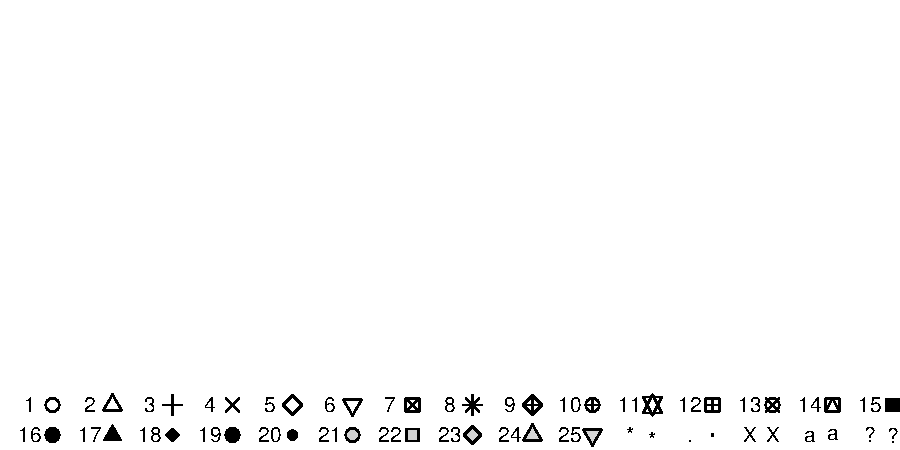
\includegraphics[width=8.5cm]{pch_symbol}

%\bcode{ps}  an integer which controls the size in points of texts and symbols
\bcode{ps}  控制文字大小的整数,单位为磅(points)

%\bcode{pty}  a character which specifies the type of the plotting region, \code{"s"}: square, \code{"m"}: maximal
\bcode{pty}  指定绘图区域类型的字符,\code{"s"}: 正方形, \code{"m"}: 最大利用

%\bcode{tck}  a value which specifies the length of tick-marks on the axes as a fraction of the smallest of the width
%or height of the plot; if \code{tck=1} a grid is drawn
\bcode{tck}  指定轴上刻度长度的值,单位是百分比,以图形宽、高中最小一个作为基数;如果 \code{tck=1} 则绘制 grid

%\bcode{tcl}  a value which specifies the length of tick-marks on the axes as a fraction of the height of a line of text
%(by default \code{tcl=-0.5})
\bcode{tcl}  同上.但以文本行的高度为基数(默认为 \code{tcl=-0.5})

%\bcode{xaxt}  if \code{xaxt="n"} the $x$-axis is set but not drawn (useful in conjonction with \code{axis(side=1, ...)})
\bcode{xaxt}  如果 \code{xaxt="n"} 则设置 $x$-轴 但不显示 (有助于和\code{axis(side=1, ...)}一起使用)

%\bcode{yaxt}  if \code{yaxt="n"} the $y$-axis is set but not drawn (useful in conjonction with \code{axis(side=2, ...)})
\bcode{yaxt}  同上. $y$-轴




%\section{Lattice (Trellis) graphics}
\section{网格(Lattice)绘图}
\everypar={\hangindent=9mm}

%\bcode{xyplot(y\~{}x)}  bivariate plots (with many functionalities)
\bcode{xyplot(y\~{}x)}  双变量散点图

%\bcode{barchart(y\~{}x)}  histogram of the values of \code{y} with
%respect to those of \code{x}~\bcode{barchart(y\~{}x)}  \code{y} 对 \code{x}~的条形图

%\bcode{dotplot(y\~{}x)}  Cleveland dot plot (stacked plots line-by-line
%and column-by-column)
\bcode{dotplot(y\~{}x)}  Cleveland 点图 (逐行逐列累加图)

%\bcode{densityplot(\~{}x)}  density functions plot
\bcode{densityplot(\~{}x)}  密度函数图

%\bcode{histogram(\~{}x)}  histogram of the frequencies of \code{x}~\bcode{histogram(\~{}x)}  \code{x}~的频率直方图

%\bcode{bwplot(y\~{}x)}  'box-and-whiskers' plot
\bcode{bwplot(y\~{}x)}  箱线图

%\bcode{qqmath(\~{}x)}  quantiles of \code{x}~with respect to the values expected under a theoretical distribution
\bcode{qqmath(\~{}x)}   \code{x}~关于某理论分布的分位数-分位数图

%\bcode{stripplot(y\~{}x)}  single dimension plot, \code{x}~must be numeric, \code{y} may be a factor
\bcode{stripplot(y\~{}x)}  一维图,\code{x}~必须是数值型, \code{y}可以是因子

%\bcode{qq(y\~{}x)}  quantiles to compare two distributions, \code{x}~must be numeric,
%\code{y} may be numeric, character, or factor but must have two 'levels'
\bcode{qq(y\~{}x)}  比较两个分布的分位数, \code{x}~必须是数值型, \code{y}可以是数值,字符或者是因子,但必须是两个'水平'

%\bcode{splom(\~{}x)}  matrix of bivariate plots
\bcode{splom(\~{}x)}  二维图矩阵

%\bcode{parallel(\~{}x)}  parallel coordinates plot
\bcode{parallel(\~{}x)}  平行坐标图

%\bcode{levelplot(z\~{}x*y|g1*g2)}  coloured plot of the values of \code{z} at the coordinates
%given by \code{x}~and \code{y} (\code{x}~, \code{y} and \code{z} are all of the same length)
\bcode{levelplot(z\~{}x*y|g1*g2)}  在 \code{x}~,\code{y} 坐标点的 \code{z} 值的彩色等值线图
(\code{x}~,\code{y}和\code{z}等长)

%\bcode{wireframe(z\~{}x*y|g1*g2)}  3d surface plot
\bcode{wireframe(z\~{}x*y|g1*g2)}  3d 透视图(面)

%\bcode{cloud(z\~{}x*y|g1*g2)}  3d scatter plot
\bcode{cloud(z\~{}x*y|g1*g2)}  3d透视图(点)

\everypar={\hangindent=0mm}
%In the normal Lattice formula, \code{y~x|g1*g2} has
%combinations of optional conditioning variables \code{g1}
%and \code{g2} plotted on separate panels.
在一般性 Lattice 公式中, \code{y\~{}x|g1*g2} 有可选择条件变量 \code{g1} 和 \code{g2} 组合绘制在单独的 'panels'上.
%Lattice functions take many of the same arguments as base
%graphics plus also \code{data=} the data frame for the formula
%variables and \code{subset=} for subsetting. Use \code{panel=} to
%define a custom panel function (see \code{apropos("panel")}
%and \code{?llines}).
Lattice 函数使用了很多相同的参量作为基础附加绘图,如 \code{data=},\code{subset=}.
使用 \code{panel=} 来定义定制'panel'函数(参考 \code{apropos("panel")}和 \code{?llines}).
%Lattice functions return an object of class
%trellis and have to be \code{print}-ed to produce the graph. Use
%\code{print(xyplot(...))} inside functions where automatic
%printing doesn't work.
Lattice 函数返回一个 trellis 类型的对象并且是'\code{print}-ed'来生成图形.
内部使用\code{print(xyplot(...))}函数时,自动绘图并无效果.
%Use \code{lattice.theme} and \code{lset} to change Lattice defaults.
使用 \code{lattice.theme} 和 \code{lset} 来改变 Lattice 默认设置.


%\section{Optimization and model fitting}
\section{模型拟和}
\everypar={\hangindent=9mm}

%\bcode{optim(par, fn, method = c("Nelder-Mead", "BFGS", "CG",
%  "L-BFGS-B", "SANN")} general-purpose optimization; \code{par} is
%  initial values, \code{fn} is function to optimize (normally minimize)
\bcode{optim(par, fn, method = c("Nelder-Mead", "BFGS", "CG",
  "L-BFGS-B", "SANN")}  用于求多元函数的最值.基于 Nelder-Mead, quasi-Newton and conjugate-gradient算法.
  同时,也可以求区间内的最值.\code{par} 为函数初值,
  \code{fn} 是求最值的函数(通常为最小)

%\bcode{nlm(f,p)} minimize function \code{f} using a Newton-type
%algorithm with starting values \code{p}
\bcode{nlm(f,p)} 根据初始值通过使用牛顿(Newton-type)算法的最小化函数

%\bcode{lm(formula)} fit linear models; \code{formula} is typically of
%     the form \code{response ~termA + termB + ...}; use \code{I(x*y)
%     + I(x\^{}2)} for terms made of nonlinear components
\bcode{lm(formula)} 拟和线性模型; \code{formula}的典型形式为 \\
 \code{response \~{} termA + termB + ...};
使用 \code{I(x*y) + I(x\^{}2)} 来构成非线性成分

%\bcode{glm(formula,family=)} fit generalized linear models, specified by
%     giving a symbolic description of the linear predictor and a
%     description of the error distribution; \code{family} is a
%     description of the error distribution and link function to
%          be used in the model; see \code{?family}
\bcode{glm(formula,family=)} 通过指定线性预测模型和残差分布来拟和广义线性模型;
\code{family}为残差分布的描述且同模型整合;详见{?family}



%\bcode{nls(formula)} nonlinear least-squares estimates of the nonlinear
%     model parameters
\bcode{nls(formula)} 非线性最小二乘估计

%\bcode{approx(x,y=)} linearly interpolate given data points; \code{x}~can be an
%xy plotting structure
\bcode{approx(x,y=)} 线性插值;

\bcode{approxfun(x,y)}  线性插值函数

%\bcode{spline(x,y=)} cubic spline interpolation
\bcode{spline(x,y=)} 立方(曲线)插值

\bcode{splinefun(x,y)} 立方(曲线)插值函数

%\bcode{loess(formula)} fit a polynomial surface using local fitting
\bcode{loess(formula)} 局部近似回归。利用局部加权回归进行一个非参回归。
这种回归对显示一组凌乱数据的趋势和描述大数据集的整体情况非常有用。

%\everypar={\hangindent=0mm}
%Many of the formula-based modeling functions have several common
%arguments: \code{data=} the data frame for the formula variables,
%\code{subset=} a subset of variables used in the fit,
%\code{na.action=} action for missing values: \code{"na.fail"}, \code{"na.omit"}, or
%a function. The following generics often apply to model fitting functions:
\everypar={\hangindent=0mm}
很多以公式为基础的模型函数有很多通用的参量: \code{data=} 公式变量的数据框, \code{subset=} 满足条件的子集;
\code{na.action=} 缺失值处理方式:\code{"na.fail"},\code{"na.omit"}, 或一个函数.
下面常用于模型拟和函数:

\everypar={\hangindent=9mm}
%\bcode{predict(fit,...)}  predictions from\code{fit} based on input data
\bcode{predict(fit,...)}  通过拟和模型\code{fit} 计算预测值

%\bcode{df.residual(fit)}  returns the number of residual degrees of freedom
\bcode{df.residual(fit)}  返回残差的自由度

%\bcode{coef(fit)}  returns the estimated coefficients (sometimes with their standard-errors)
\bcode{coef(fit)}  返回被估计的系数(有时候还包括他们的标准差 )

%\bcode{residuals(fit)}  returns the residuals
\bcode{residuals(fit)}  返回残差值

%\bcode{deviance(fit)}  returns the deviance
\bcode{deviance(fit)}  返回方差

%\bcode{fitted(fit)}  returns the fitted values
\bcode{fitted(fit)}  返回拟和值

%\bcode{logLik(fit)}  computes the logarithm of the likelihood and the number of parameters
\bcode{logLik(fit)}  计算对数似然值和参数数目

%\bcode{AIC(fit)}  computes the Akaike information criterion or AIC
\bcode{AIC(fit)}  计算~Akaike~信息准则(Akaike information criterion or AIC)

%\section{Statistics}
\section{统计}
\everypar={\hangindent=9mm}

%\bcode{aov(formula)} analysis of variance model
\bcode{aov(formula)} 方差分析

%\bcode{anova(fit,...)} analysis of variance (or deviance) tables for one or more
%     fitted model objects
\bcode{anova(fit,...)} 一个或多个模型对象的方差表(或残差平方和表)分析

%\bcode{density(x)} kernel density estimates of\code{x}~\bcode{density(x)}\code{x}~的核密度估计

\bcode{kmeans(x)}   ~k~均值聚类

\bcode{hclust(d, method = "complete")} 层次聚类分析,~d~由函数~dist~构造,\code{method} 可参考 ?hclust

\bcode{prcomp(x, ...)}  主成分分析

%\bcode{factanal(x,factors,data)}    Perform maximum-likelihood factor analysis on a covariance matrix or data matrix.
\bcode{factanal(x,factors,data)}    因子分析

%\bcode{cancor(x, y, xcenter = TRUE, ycenter = TRUE)}       Compute the canonical correlations between two data matrices.
\bcode{cancor(x, y, xcenter = TRUE, ycenter = TRUE)}   典型相关分析( canonical correlations )


%\bcode{binom.test()}, \bcode{pairwise.t.test()}, \bcode{power.t.test()},

%\bcode{prop.test()}, \bcode{t.test()}, ... 使用
%\code{help.search("test")}

%%%%%%%%%%%%%%%%%%%%%%%
%%%2007-1-20
%%%test
%%%%%%%%%%%%%%%%%%%%%%%%
\section{检验}
\bcode{t.test()}  $t$检验

\bcode{wilcox.test()} ~Wilcoxon~检验

\bcode{prop.test(x,n,p)}   n次试验中,出现的x的概率是否以概率~p~出现的假设检验

\bcode{binom.test(x,n)} 贝努力试验检验

\bcode{chisq.test(x,p)}  $\chi^2$检验

\bcode{fisher.test(x ,y = NULL)} Fisher 精确性检验

\bcode{ks.test(x,y="name",)}    Kolmogorov-Smirnov检验,检验向量数据是否服从"name"分布

\bcode{shapiro.test(x)}    Shapiro-Wilk正态分布检验

\bcode{PP.test(x, lshort = TRUE)} PP(Phillips-Perron)检验

\bcode{quada.test(x)}   ~quade~检验

\bcode{friedman.test(x)}    ~Friedman~秩和检验


\bcode{pairwise.t.test()}, \bcode{power.t.test()}

\code{help.search("test")}

%\section{Distributions}
\section{分布}

%\bcode{rnorm(n, mean=0, sd=1)} Gaussian (normal)
\bcode{rnorm(n, mean=0, sd=1)} 高斯 (正态)

%\bcode{rexp(n, rate=1)} exponential
\bcode{rexp(n, rate=1)} 指数

%\bcode{rgamma(n, shape, scale=1)} gamma
\bcode{rgamma(n, shape, scale=1)} $\gamma$ 分布

%\bcode{rpois(n, lambda)} Poisson
\bcode{rpois(n, lambda)} Poisson 分布

%\bcode{rweibull(n, shape, scale=1)} Weibull
\bcode{rweibull(n, shape, scale=1)} Weibull 分布

%\bcode{rcauchy(n, location=0, scale=1)} Cauchy
\bcode{rcauchy(n, location=0, scale=1)} Cauchy 分布

%\bcode{rbeta(n, shape1, shape2)} beta
\bcode{rbeta(n, shape1, shape2)} $\beta$ 分布

%\bcode{rt(n, df)} 'Student' ($t$)
\bcode{rt(n, df)} $t$分布

%\bcode{rf(n, df1, df2)} Fisher--Snedecor ($F$)  ($\chi^2$)
\bcode{rf(n, df1, df2)} F 分布

%\bcode{rchisq(n, df)} Pearson
\bcode{rchisq(n, df)} $\chi^2$分布

%\bcode{rbinom(n, size, prob)} binomial
\bcode{rbinom(n, size, prob)} 二项

%\bcode{rgeom(n, prob)} geometric
\bcode{rgeom(n, prob)} 几何

%\bcode{rhyper(nn, m, n, k)} hypergeometric
\bcode{rhyper(nn, m, n, k)} 超几何

%\bcode{rlogis(n, location=0, scale=1)} logistic
\bcode{rlogis(n, location=0, scale=1)} logistic 分布

%\bcode{rlnorm(n, meanlog=0, sdlog=1)} lognormal
\bcode{rlnorm(n, meanlog=0, sdlog=1)} 对数正态

%\bcode{rnbinom(n, size, prob)} negative binomial
\bcode{rnbinom(n, size, prob)} 负二项分布

%\bcode{runif(n, min=0, max=1)} uniform
\bcode{runif(n, min=0, max=1)} 均匀分布

%\bcode{rwilcox(nn, m, n)},\code{rsignrank(nn, n)} Wilcoxon's statistics
\bcode{rwilcox(nn, m, n)},\code{rsignrank(nn, n)} Wilcoxon 分布

%All these functions can be used by replacing the letter\code{r} with
%\code{d},\code{p} or\code{q} to get, respectively, the probability
%density (\code{d\textsl{func}(x, ...)}), the cumulative probability
%density (\code{p\textsl{func}(x, ...)}), and the value of quantile
%(\code{q\textsl{func}(p, ...)}, with 0 $<$\code{p} $<$ 1).
所有的函数都可以使用\code{d},\code{p} 或\code{q} 来替换\code{r}
分别得到概率密度 (\code{dfunc(x, ...)}), 累积概率密度
 (\code{pfunc(x, ...)}), 分位数 (\code{qfunc(p, ...)},
 0 $<$\code{p} $<$ 1).



%\section{Programming}
\section{编程}
\everypar={\hangindent=9mm}

%\bcode{function( arglist ) expr} function definition
\bcode{function( arglist ) expr} 定义函数

\bcode{return(value)}

\everypar={\hangindent=0mm}
\bcode{if(cond) expr\\
if(cond) cons.expr  else  alt.expr\\
for(var in seq) expr\\
while(cond) expr\\
repeat expr\\
break\\
next}

%Use braces \{\} around statements
使用表达(statements)使用大括号 \{\}

\everypar={\hangindent=9mm}
%\bcode{ifelse(test, yes, no)} a value with the same shape as\code{test} filled with elements
%from either\code{yes} or\code{no}
\bcode{ifelse(test, yes, no)} 如果满足条件\code{test}返回\code{yes},反之返回\code{no}

%\bcode{do.call(funname, args)} executes a function call from the name of
%  the function and a list of arguments to be passed to it
\bcode{do.call(funname, args)} 根据函数名和表达式(arguments)执行调用函数.


\section{R~内嵌常数}
\everypar={\hangindent=9mm}
\bcode{letters}   返回26个小写英文字母

\bcode{LETTERS}  同上(大写)

\bcode{month.abb}    返回3个字母缩写的月份名

\bcode{month.name}   返回月份名

\bcode{pi}  $\pi$

\section{其他}
\everypar={\hangindent=9mm}
%\bcode{sessionInfo()}  Print version information about R and attached packages.
\bcode{sessionInfo()}  显示关于~R~的版本信息和关联的~Packages

%\bcode{all.equal(x,y)}  Test if Two Objects are (Nearly) Equal
\bcode{all.equal(x,y)}  检验两个对象是否(渐进)相等,相等返回 TRUE,否则返回$abs(x-y)/x$

%\bcode{identical} Test Objects for Exact Equality
\bcode{identical(x,y)} 严格检验对象是否相等

\bcode{memory.size()}   返回当前使用的内存大小

\bcode{RSiteSearch()}   搜索\url{http://search.r-project.org}上的结果,包括邮件列表,手册和帮助页



\end{multicols*}
\end{document}
